% Chapter Intro

\chapter{Measurement of the CENNS with Cryogenic Bolometers in the \Ricochet{} experiment} % Main chapter title

\label{ChapterIntro} % Change X to a consecutive number; for referencing this chapter elsewhere, use \ref{ChapterX}

%----------------------------------------------------------------------------------------
%	BEGING CHAPTER
%----------------------------------------------------------------------------------------

\section{CE$\nu$NS and the new physics}

\subsection{Coherent Elastic Neutrino-Nucleus Scattering}

A scattering phenomenon occurs when two particles interacts during a collision.
%A scattering is considered to be elastic when the energies of the two particles are conserved trough the collision, even though their momentum is not necessarily preserved. 
An elastic scattering is a process where the kinetic energy of a particle is conserved in the center-of-mass frame, but its direction of propagation is modified (by interaction with other particles and/or potentials). Furthermore, while the particle's kinetic energy in the center-of-mass is constant, its energy in the lab frame is not.
This work especially focuses on the elastic scattering between neutrinos and atomic nuclei. Even though the nucleus is an assembly of nucleons, a coherent scattering occurs when the neutrino can interact with the nucleus as a whole, as if it was a uniform object.
When the scattering of a neutrino on a nucleus is coherent and elastic, it is defined as a Coherent Elastic Neutrino-Nucleus Scattering, shortened to CE$\nu$NS or CENNS.
This physical phenomenon, described by Freedman in 1973 within the framework of the Standard Model, was  measured for the first time in august of 2017 by the COHERENT collaboration, with an experiment installed near the spallation source at the Oak Ridge National Laboratory in the United States.
Before presenting the scientific context of this work, a brief recall is done on nucleus and neutrino. We will therefore discuss the CENNS equations and the various experiments aimed at measuring this process.


\subsection{The Atomic Nucleus}

Rutherford's experience with gold leaf in 1909 provided valuable information for the development of Bohr's atomic model in 1913. Rutherford understood that the electrically positively charged of an atom is concentrated in the middle of the atom. Indeed, knowing that the matter is electrically neutral and that an atom has electrons (charged negatively) there are necessarily positive charges "somewhere". Bohr then designed an atomic model for the hydrogen that reminds us of a planetary system. There would be the nucleus at the center and the electrons around it, only allowed to be on specific circular orbitals.
Theoretical and experimental developments show us today that the electrons are not really on circular orbits but rather have a probability of presence described by combinations of spherical harmonics. Bohr's model for hydrogen is not fundamentally questioned and is still taught. Electrons are considered to orbit around the nucleus of positive charge. The latter can be either stable or unstable in the case of radioactive elements. 
This is an important fact, that an atom is not a fundamental object of modern physics: it is composed of nucleons (neutrons and protons), which are themselves composed of three quarks held together by to the strong nuclear interaction mediated by gluons. The size of an atom is of the order of $\SI{0.1}{\nano\m} = \SI{e-10}{\m}$ which is five orders of magnitude larger than the size of its nucleus $\SI{1}{\femto\m} = \SI{e-15}{\m}$.


\subsection{The Neutrino}

The neutrino is one of the elementary particles of the Standard Model (SM) of particles physics, which is an electrically neutral lepton. There are three flavors of neutrinos each associated with a charged lepton: the electronic neutrino $\nu_e$ is coupled to the electron $e^-$, the muonic neutrino $\nu_{\mu}$ with the muon $\mu^-$ and the tauic neutrino $\nu_{\tau}$ with the tau $\tau^-$.
The physicist Wolfgang Pauli was the first to postulate the existence of the neutrino in 1930. This new particle (at the time) helped to explain the continuous spectrum of the beta disintegration, which is a radioactive decay in which a radionucleide emits an electron (or positron) and an antineutrino (or neutrino).
The experimental confirmation was obtained by Cowan and Reines in 1956 based on an idea by Wang Ganchang (1942) and Reines was awarded the Nobel Prize for physics in 1995 for this discovery.
A neutrino is only sensitive to the electroweak and gravitational interactions. The later is negligible in particle physics but hold impact on the larger scale of cosmology. 
%Due to the short range of the weak interaction (\SI{e-18}{\m}) 
The neutrino has a very low probability of interaction with matter, which is formalized in particle physics as a weak cross-section. To have an order of magnitude in mind we can show that out of 10 billion neutrinos of \SI{1}{\mega\eV} that cross the Earth, only 1 will interact with its components.
In the study of the CENNS process, no particular attention is brought on distinguishing  neutrinos from antineutrinos as well as different flavors. Indeed, this scattering process is insensitive to these differences. 


\subsection{CENNS and Standard Model}

It was in 1973 that Daniel Z. Freedman, a physicist currently at MIT, proposed the coherent elastic neutrino-nucleus scattering as a probe for weak interaction \cite{Freedman:1973yd}.
 In its description based on the Standard Model still under development at that time (it will take its current form in the mid-1970s), Freedman expresses the evolution rate of the effective cross-section of the neutrino-nucleus interaction as a function of the recoil energy of the nucleus:
\begin{equation}
\label{eq:cenns-equation}
\frac{\mathrm{d} \sigma (E_{\nu}, E_R)}{\mathrm{d} E_R}
=
\frac{G_{f}^2}{4\pi}
Y_w^2  m_A
\left( 1 - \frac{m_A E_R}{2 E_{\nu}^2} \right)
F^2(E_r)
\end{equation}
This equation shows that the evolution of the effective cross-section noted $\sigma(E_{\nu} , {E_R} )$ depends on the neutrino energy $E_{\nu}$ and recoil energy $E_r$ of the nucleus as well as of the mass of the target nucleus $m_A$. Without going into the details of the theoretical calculations to obtain this expression, one can try to explain simply the different terms.

The Fermi coupling constant $G_f$ is measured experimentally by studying  the life time of the muon (inversely proportional to $G_f^2$) \cite{Chitwood:2007}.
We can express $G_f$ with the coupling constant of the weak interaction $g_W$ , the mass $m_W$ of the boson W, the speed of light $c$ and the reduced Planck constant $\hbar$ according to the equation:
\begin{equation}
G_f 
=
\frac{\sqrt{2}}{8}
\left( \frac{g_W}{m_W c^2} \right)^2
(\hbar c)^3
\sim \SI{1.17e-5}{\giga \eV^{-2}}
\end{equation}

The weak nuclear hypercharge $Y_w$ is given by:
\begin{equation}
Y_w = N - Z (1 - 4 \sin^2 \theta_w)
\end{equation}
It depends on the number of neutrons $N$ and protons $Z$ composing the nucleus. The term  $\theta_w$ is the mixing angle which is a parameter of the Weinberg-Salam theory of the electroweak interaction (reunification of the theory of electromagnetism and weak interaction).
The value of $\sin^2 \theta_w$ is close to 0.24 \cite{Cadeddu:2018izq}. 
Thus, in practice, the hypercharge simplifies to $Y_w \simeq N$. As described later in this work, the measurement of the $\sin^2 \theta_w$ value as a function of the transferred momentum would permit to probe for new physics in the electroweak sector.

The form factor $F$ is a function of the recoil energy that characterizes the loss of coherence at high transferred momentum. It is equal to 1 for low recoil energies, so it is often neglected in very low energy regimes, and decreases with the recoil energy $E_R$.

% (total)
The effective cross-section $\sigma$ associated with the CENNS is obtained by integrating the equation \ref{eq:cenns-equation} from $E_R = 0$ to $E_R^{max} = 2E_{\nu}^2 / (m_A + 2E_{\nu} )$, the maximum recoil energy of the nucleus accessible for a given neutrino energy $E_{\nu}$ \cite{Scholberg:2015}.
Its expression is:
\begin{equation}
\sigma
\sim
\frac{G_f^2 N^2}{4\pi} E_{\nu}^2
\end{equation}
which is proportional to the square of the number of neutrons $N$ in the target nucleus and the energy of the neutrino thanks to the coherence of the interaction in case $m_N \gg E_{\nu}$.

The detection of CENNS is not done by directly measuring the cross-section of the particles that interact with the atomic nuclei of the detector. We measure the number of neutrinos having interacted with a nucleus according to the recoil energy of the latter. By doing this on a fairly wide range of recoil energy, we end up with what is called an energy spectrum of CENNS events. In this case, we will speak of CENNS spectrum, and of energy spectrum in the general case for different scattering processes. The expected differential CENNS event rate $R$ is calculated from the differential cross-section by convolving with the incoming neutrino flux $\Phi$:
\begin{equation}
\frac{\mathrm{d} R}{\mathrm{d} E_r}
=
\mathcal{N}
\int_{E_{\nu}^{min}}
\Phi(E_{\nu})
\frac{\mathrm{d} \sigma (E_{\nu}, E_r) }{\mathrm{d} E_r} \mathrm{d} E_{\nu}
\end{equation}
In this equation, $\mathcal{N}$ represents the number of target nuclei per mass unit. The minimum energy of a neutrino to induce a nuclear recoil is given by the relation $E_{\nu}^{min}= \sqrt{m_N E_R /2}$.

A common representation of this type of interaction in particle physics is done with the help of Feynman diagrams. In this representation, the time flows from left to right and the distance between the particles is represented along the vertical axis. The mediator bosons are indicated with wavy lines. The figure \ref{fig:cenns-feynman} displays two Feynman diagrams for the CENNS.
\begin{figure}
\centering
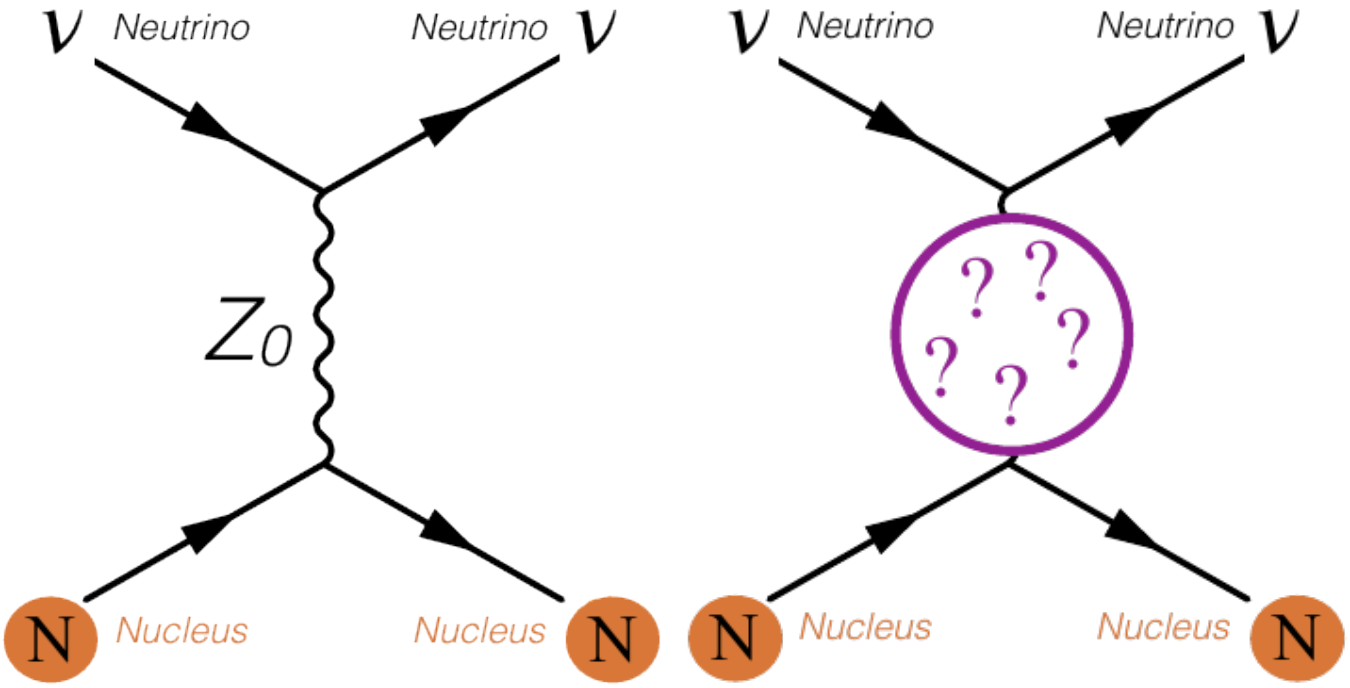
\includegraphics [scale=1]{Figures/Introduction/cenns_feynman.png}
\caption{Feynman diagrams of the CEvNS. On the left in the case of the Standard Model. On the right the same process within the framework of alternative theories.}
\label{fig:cenns-feynman}
\end{figure}
The left diagram corresponds to the CENNS process in the SM framework, by having the $Z_0$ boson as the mediator of the weak interaction between the neutrino and the nucleus. The right diagram presents the CENNS in the framework of alternative theories.


\subsection{First Detection of CE$\nu$NS}

The COHERENT collaboration was the first to observe experimentally and unambiguously the signature of the CENNS in August 2017 \cite{Akimov:2017bs}.
The technology used at that time was a \SI{14.6}{\kg} sodium-doped cesium iodide (\ce{CsI[Na]}) scintillator instrumented with photo-multipliers. The detector was located at a distance of \SI{19.3}{\m} from the neutrino source and had an energy detection threshold of \SI{4.5}{\kilo\eV}. The neutrino flux of average energy $E_{\nu} = \SI{30}{\mega\eV}$ used for this detection was produced with the so-called "pion-at-rest" method. It consists in taking advantage of the decay of positive pions, obtained after a controlled collision of a mercury atom with a proton, which leads to the production of neutrinos and antineutrinos. The proton source comes from the SNS (Spallation Neutron Source) located at the Oak Ridge National Laboratory in Oak Ridge, Tennessee (USA). 

Scientists in the collaboration have detected an excess of CENNS-like events, shown in Figure \ref{fig:coherent-result}, with a confidence level of $6.7\sigma$ compatible at $1\sigma$ with the SM prediction. The statistical uncertainty of this study is estimated to \SI{16}{\percent}. This result proves the existence of the CENNS process which has been considered for years as purely hypothetical.

\begin{figure}
\centering
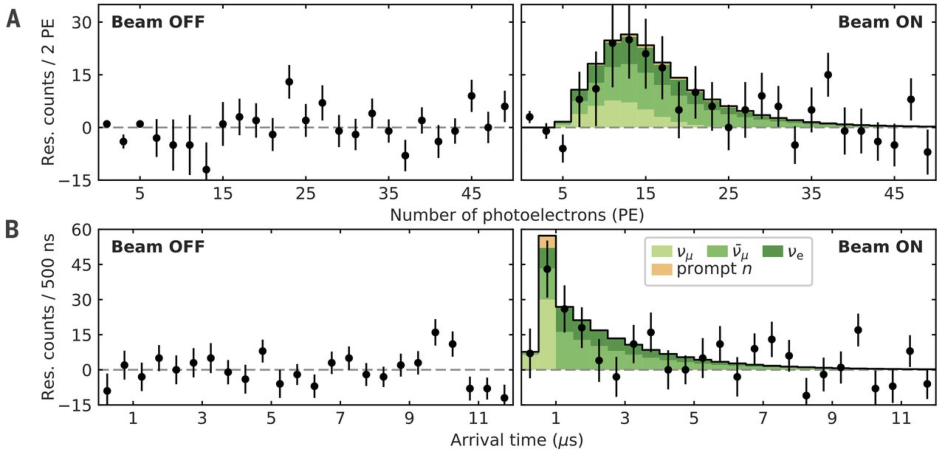
\includegraphics [scale=1]{Figures/Introduction/coherent_result.pdf}
\caption{Experimental result of the COHERENT experiment at the SNS demonstrating unambiguously the existence of the CENNS. Figure taken from \cite{Akimov:2017bs}.}
\label{fig:coherent-result}
\end{figure}

It would be now possible to constrain models of new physics \cite{Akimov:2017bs}. Nevertheless current data do not allow to study predictions in the low-energy region such as the existence of new mediating bosons \cite{Billard:2018jnl}. This requires a source of lower energy neutrinos, which in turn requires detectors with lower energy threshold.


\section{Search for New Low Energy Physics}

%A number of theories diverge significantly from the prediction of the Standard Model at low energy. Among them we can mention in particular :
In the framework of beyond Standard Model physics, the measure of the CENNS process at low-energy could be associated with:
\begin{itemize}
	\item the existence of new massive bosons,
	\item the existence of an anomalously large magnetic moment of the neutrino,
	\item the existence of non-standard interactions.
\end{itemize}

There is an important scientific stake in making these low energy measurements to provide additional elements in the understanding of fundamental interactions but also to provide additional constraints for a large number of neutrino research projects. A precise measurement of the CENNS would, for example, make it possible to constrain the previously mentioned theoretical models. 

However, to do new physics research with the CENNS process, the use of a suitable neutrino source is required. This source should have a known and adapted neutrino energy spectrum (typically $E_{\nu} \approx \SI{10}{\mega\eV}$). This will result in lowered recoil energies $E_R$ in the detector requiring lower energy threshold. This upgrade in detector performances can only be reached by diminishing the volume of the detectors resulting in a loss of exposure. As such, the neutrino source should produce a very high flux of neutrinos as to counter the inevitable loss of detector mass and obtain an equivalently high CENNS event rate.

Additionally, various technical and practical considerations are taken into account: possibility of interruption of the flow (or pulsed flow) for background rejection (as in the case of COHERENT for example), minimum accessible source/detector distance, ease of access and installation, regulations and availability of infrastructure.

\subsection{Neutrino Sources}

There are many sources of neutrinos because the radioactive decay processes that generate them are very common in nature. This subsection discusses some common low-energy neutrino sources and their characteristics regarding the search for CENNS. Neutrinos out of experimental range such as those composing the cosmic neutrino background (the analogue of the cosmic microwave background for neutrinos) or the diffuse supernovae neutrino background will not be discussed. The resting pion method used by COHERENT will not be recalled as it has already been presented and is not a viable solution for the search for new low energy physics because of the too large energy of the emitted neutrinos and too low integrated flux.

\subsubsection{Solar Neutrinos}

Thermonuclear fusion reactions take place in the heart of stars. During these reactions, low energy neutrinos (a few \si{\mega\eV}) are emitted. They escape from their original star without great difficulty thanks to their low effective cross-section. The process responsible for most of the neutrino emission of the Sun, is the fusion of two protons \ce{p} into a \ce{^2H} deuterium (heavy hydrogen) nucleus, an anti-electron \ce{e^+} (otherwise known as positron) and an electronic neutrino \ce{\nu_e}:
\begin{equation}
\ce{ p + p -> {}^2H + e^+ + $\nu$_e }
\end{equation}
For this specific reaction the energy of the emitted neutrinos is in the order of $\mathcal{O}(100)$ \si{\kilo\eV}. It should be noted, however, that there are other reactions of a different nature producing neutrinos within the Sun. The figure \ref{fig:solar-neutrino-spectrum} displays on the left, the simulated spectrum of the neutrino flux as seen from Earth associated with these different processes.
Despite of the rather large neutrino flux of the order of \SI{7e10}{\cm^{-2} \s^{-1}}, their small interaction cross-section with matter makes their detection very difficult.
% Taking all energies together, the flux of solar neutrinos at Earth is of the order of \SI{7e10}{\cm^{-2} \s^{-1}} which is relatively small and makes the detection of solar neutrinos very difficult.

\begin{figure}
\begin{minipage}{0.48\textwidth}
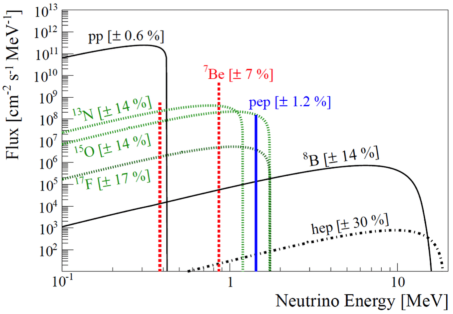
\includegraphics [scale=1]{Figures/Introduction/solar_neutrino_spectrum_simu.pdf}
\end{minipage}
\hfill
\begin{minipage}{0.48\textwidth}
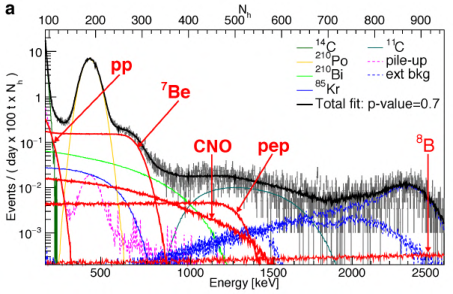
\includegraphics [scale=1]{Figures/Introduction/solar_neutrino_spectrum_exp.pdf}
\end{minipage}
\caption{Solar neutrino spectrum. On the left, simulated spectra of solar neutrinos seen from the Earth associated with the different fusion reactions, taken from \cite{DAngelo:2014lmb}.
On the right, solar neutrino spectrum and its components measured by the Borexino experiment at the Gran Sasso in Italy, taken from \cite{Redchuk:2020mza}.}
\label{fig:solar-neutrino-spectrum}
\end{figure}

Despite this difficulty, large experiments, such as Borexino located in the underground laboratory of the Gran Sasso in Italy, are able to measure this solar neutrino spectrum as seen on the right subplot of figure \ref{fig:solar-neutrino-spectrum}. However, for a CENNS precision measurement experiment, the Sun is clearly not a relevant source because even if the energy of some neutrinos is low enough for probing new physics, the neutrino flux is too low and would require a huge volume (mass) of detector as used by solar neutrino experiments as SNO \cite{Bellerive:2016}. Another negative point is that it is not possible to turn off the source to identify the background noise. Indeed, the solar neutrino flux is constant and crosses the Earth to reach the detector without difficulty.

\subsubsection{Terrestrial Neutrinos (geo-neutrinos)}

Our own planet, the Earth, emits neutrinos through natural radioactivity processes.
Geo-neutrinos are emitted by the Earth's core through natural radioactivity processes, resulting in a flux at the Earth's surface estimated to be \SI{1e6}{\cm^{-2} \s^{-1}} \cite{Bellini:2013}. This flux of geo-neutrinos is low and is coupled with a wide distribution in energy. Consequently, they are very difficult to detect because of the background of neutrinos from extraterrestrial and human origin. Nevertheless some experiments try to carry out geo-neutrino measurements for the information they would allow us to obtain on the Earth and in particular at the level of the Earth's core. The same large-scale experiment Borexino claims to have recently detected events attributable to geo-neutrinos \cite{Agostini:2020geo}.
For reasons similar to solar neutrinos, geo-neutrinos are not relevant in view of the current knowledge for CENNS precision measurement.

\subsubsection{Production from Human Activity}

Humans are capable of producing neutrinos in controlled physical processes. In particle accelerators, for example, it is not uncommon to produce neutrinos with energies of up to \SI{100}{\giga\eV}. The most intense man-made source of low-energy neutrinos are the nuclear fission power plants. However, the main objective of these power generation plants is not the production of neutrinos, which consists in a very abundant by-product of the electricity production. The flow of neutrinos emitted by a standard nuclear power plant \SI{10}{\m} from the reactor is approximately equal to \SI{2e15}{\cm^{-2} \s^{-1}}, for an average neutrino energy of \SI{4}{\mega\eV}. Nuclear fission reactors offer a range of energy compatible with the research of new physics, the neutrino flux is among the most important and in addition to that it is possible to take advantage of unit outages to measure background noise. For this last point the subtraction background noise is not as optimal as with a pulsed source if the background noise is not stationary on the time scales represented by the combustion of a fuel rod but it is always an interesting plus to gain in measurement accuracy.


\subsection{Reactor Experiments}

The strong potential of nuclear power plants as sources of neutrinos has led a small number of CENNS experiments to be installed close to a reactor core around the world. The main experiments searching for the CENNS near nuclear reactors are identified on the atlas displayed in figure \ref{fig:cenns-exp-atlas} and listed in the table \ref{tab:reactor-experiments} with their detector material and their localization.

\begin{figure}
\centering
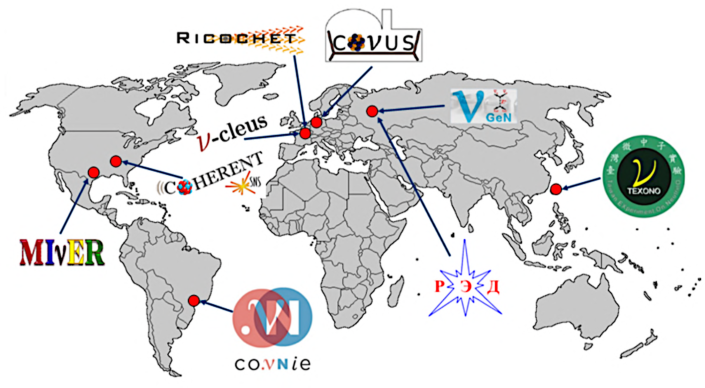
\includegraphics[scale=1]{Figures/Introduction/cenns_exp_atlas.pdf}
\caption{Main experiences of CEvNS in the world today (2020).
% Courtesy of Jules Colas
}
\label{fig:cenns-exp-atlas}
\end{figure}

\begin{table}[]
\centering
\begin{tabular}{c|c|c}
Experiment & (Detector Material) @ Location & Reference  \\ \hline \hline
NuGEN & 	(Ge) @ Kalinin Reactor (Russia) &	\cite{Belov:2015ufh} \\
CONUS & 	(Ge) @ Brokdorf (Germany) &	\cite{Lindner:2017} \\
TEXONO & 	(Ge) @ Kuo-Sheng Reactor (Taiwan) &	\cite{Soma:2016} \\
CONNIE & 	(Si) @ Angra Reactor (Brazil) & \cite{AguilarArevalo:2016} \\
RED100 & 	(Xe) @ Kalinin Reactor (Russia) &\cite{Akimov:2017} \\
MINER & 	(GeSi) @ Nuclear Science Center (USA) &	\cite{Agnolet:2016zir} \\
NU-CLEUS &	(\ce{CaWO_4}, \ce{Al_2O_3} ) @ Chooz (France) &	\cite{Strauss_2017} \\
RICOCHET & 	(Ge, Zn, Al, (Si)) @ ILL (France) &	\cite{Billard:2017giu} \\
\end{tabular}
\caption{Presentation of CENNS experiments associated with a nuclear reactor: materials used for detection @ localization. In red are represented the cryogenic experiments with a very low detection threshold for the research of new physics. The \Ricochet{} experiment is the only one to propose a detector capable of discriminating between nuclear and electronic recoils.}
\label{tab:reactor-experiments}
\end{table}

The CENNS experiments near a reactor would allow the estimation of the Weinberg angle $\theta_w$ at low energies. Figure \ref{fig:weinberg-angle} shows the SM prediction (blue line) for this parameter and the zone of the parameter space accessible by the CENNS experiments (green zone) which still remains largely unexplored. The estimation of this parameter with different physical processes is also very important to identify incompatibilities and allows the scientific community to go beyond the Standard Model.

\begin{figure}
\centering
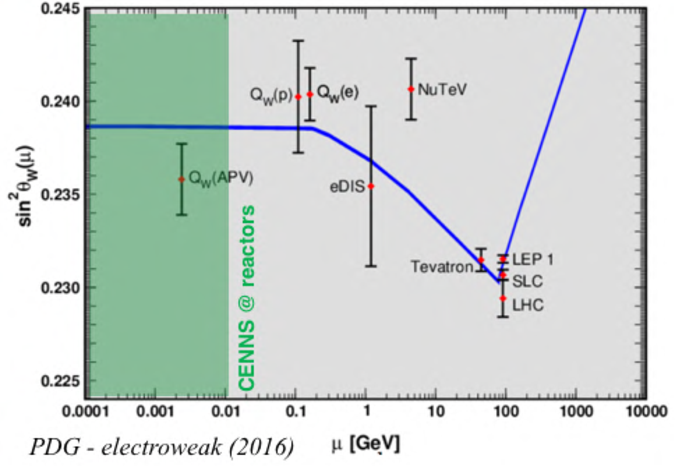
\includegraphics[scale=1]{Figures/Introduction/weinberg_angle.pdf}
\caption{Scale dependence of the weak mixing angle, adapted from \cite{Patrignani:2016xqp}. The blue curve is the prediction of the Standard Model for different processes and experiments. The green area shows the area accessible with a precision measurement of the CENNS spectrum near a nuclear reactor.}
\label{fig:weinberg-angle}
\end{figure}

In view of the number of CENNS experiments, we can expect this precision measurement within a few years. What is uncertain is whether this scientific result will deviate from the Standard Model at low-energy scale or confirm this theory. The "cooperation" at work between all these collaborations and with dark matter direct detection experiments such as \Edelweiss{} favors rapid developments and technological improvements.


\subsection{\Ricochet{}}
\label{par:cryocube}

\Ricochet{} is a CENNS experiment based on an international collaboration of
%led by the members of the MANOIR team at the \textit{Institut de Physique des deux Infinis} (IP2I) of Lyon, which brings together
some fifty researchers, technicians and engineers through various laboratories and universities in France, Russia and the United States. \Ricochet{} aims at measuring the CENNS spectrum with a statistical accuracy of \SI{1}{\percent} after one year of data taking. With this objective, the CENNS detection with low energy neutrinos (a few \si{\mega\eV}) with an accuracy of at least $5\sigma$, like the COHERENT experiment, will be reached within a week of operation. 
It should be noted that the targeted accuracy is far superior to that obtained by COHERENT. To achieve these scientific objectives the \Ricochet{} device is composed of a cryogenic system, a shielding to limit sources of unwanted background, and the CryoCube and QArray detector arrays. It will be installed in 2022 at the Laue Langevin Institute (ILL) in Grenoble, France. The ILL hosts a \SI{58}{\mega\watt} fission research nuclear reactor. A numerical modeling of \Ricochet{} at ILL and the implementation scheme near the reactor core are presented in figure \ref{fig:ricochet-ill-site}.

\begin{figure}
\centering
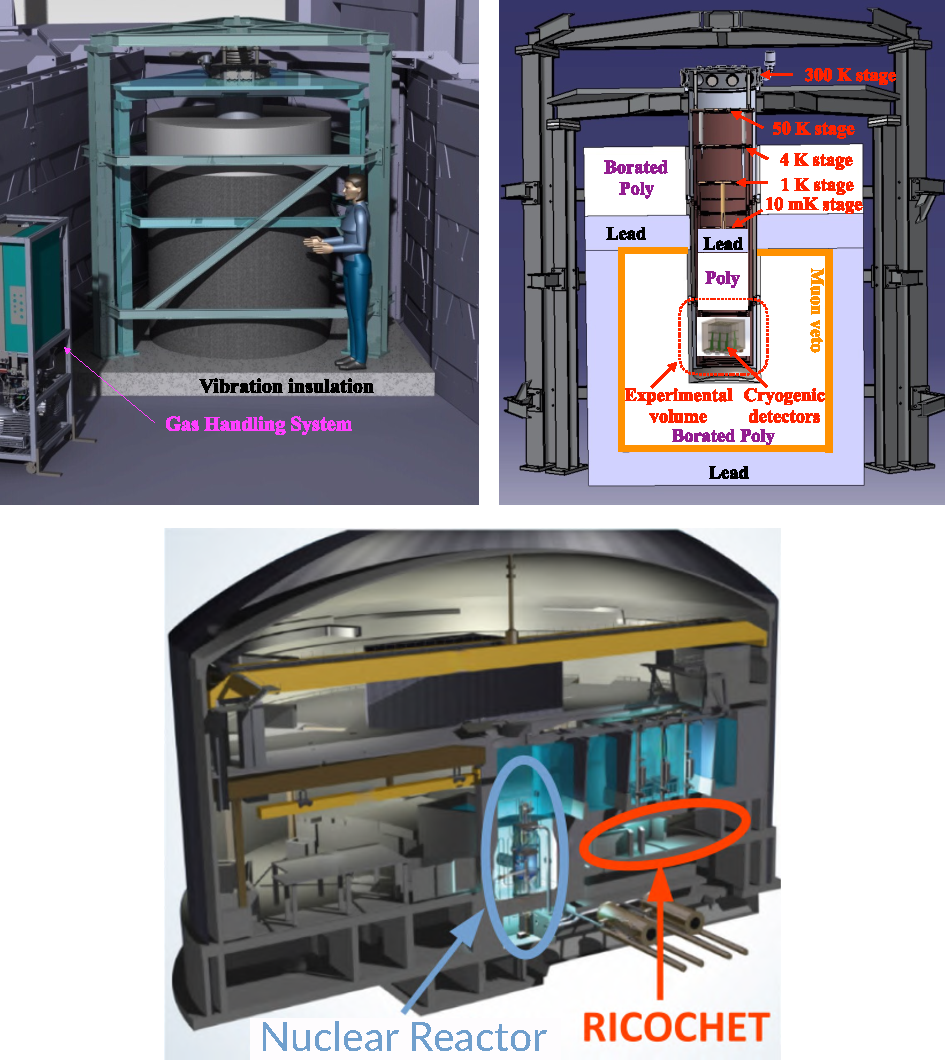
\includegraphics[scale=1]{Figures/Introduction/ricochet_ill_site.pdf}
\caption{On the top left, Installation of \Ricochet{} at ILL, 3D modeling. On the top right, view in
cryostat cut. At the bottom, location of the \Ricochet{} cryostat within the ILL nuclear reactor. The water pool above the location of \Ricochet{} provides protection against cosmic particles. Images adapted from \cite{HDRJulien}.}
\label{fig:ricochet-ill-site}
\end{figure}

The CryoCube detector will be at only \SI{8}{\m} from the core of the nuclear reactor which will produce a neutrino flux of \SI{e12}{\cm^{-2} \s^{-1}}. The CryoCube will be cooled down close to the absolute zero at cryogenic temperatures around \SI{10}{\milli\kelvin}, in order to be able to measure minute temperature rises caused by the neutrinos following their interaction with the nuclei that make up the detector's target material.

%The operation of the CryoCube detector will be detailed later. But it is necessary to know that 
The cryogenic detector load will be protected from external radiations by a thick layer of lead and borated polyethylene shielding weighting more than 15 tons and an active cosmic particle rejection device designated as "veto muon". The objective of this shielding strategy is to prevent as much as possible any unwanted diffusion processes in the experimental data which would reduce the signal-to-noise ratio and significantly hurt the chances of detecting signs of new physics.

The incident neutrino flux at the location of the CryoCube at on ILL site was estimated and
the collaboration has precisely simulated the expected CENNS spectrum according to different theoretical models considered and taking into account the different background contributions. In figure \ref{fig:cenns-new-physics}, we see the prediction of the Standard Model (in blue) and the assumed effect of two alternative theories: the existence of an anormally high magnetic moment of neutrino (violet, fine dotted line) or of a new Z' boson (violet, dashed line). The background noise, of electronic or nuclear origin, is represented in grey and is for both almost uniform in the energy range considered.

This numerical simulation allows to define the specifications of \Ricochet{} so that the CENNS spectrum is measured specifically in the region of interest for new physics search. From the spectra associated with two exotic physics scenarios in figure \ref{fig:cenns-new-physics}, we see that we need a low enough detection threshold in recoil energy. Otherwise, we will not be able to see the deviations from the Standard Model or even the CENNS itself.

\begin{figure}
\centering
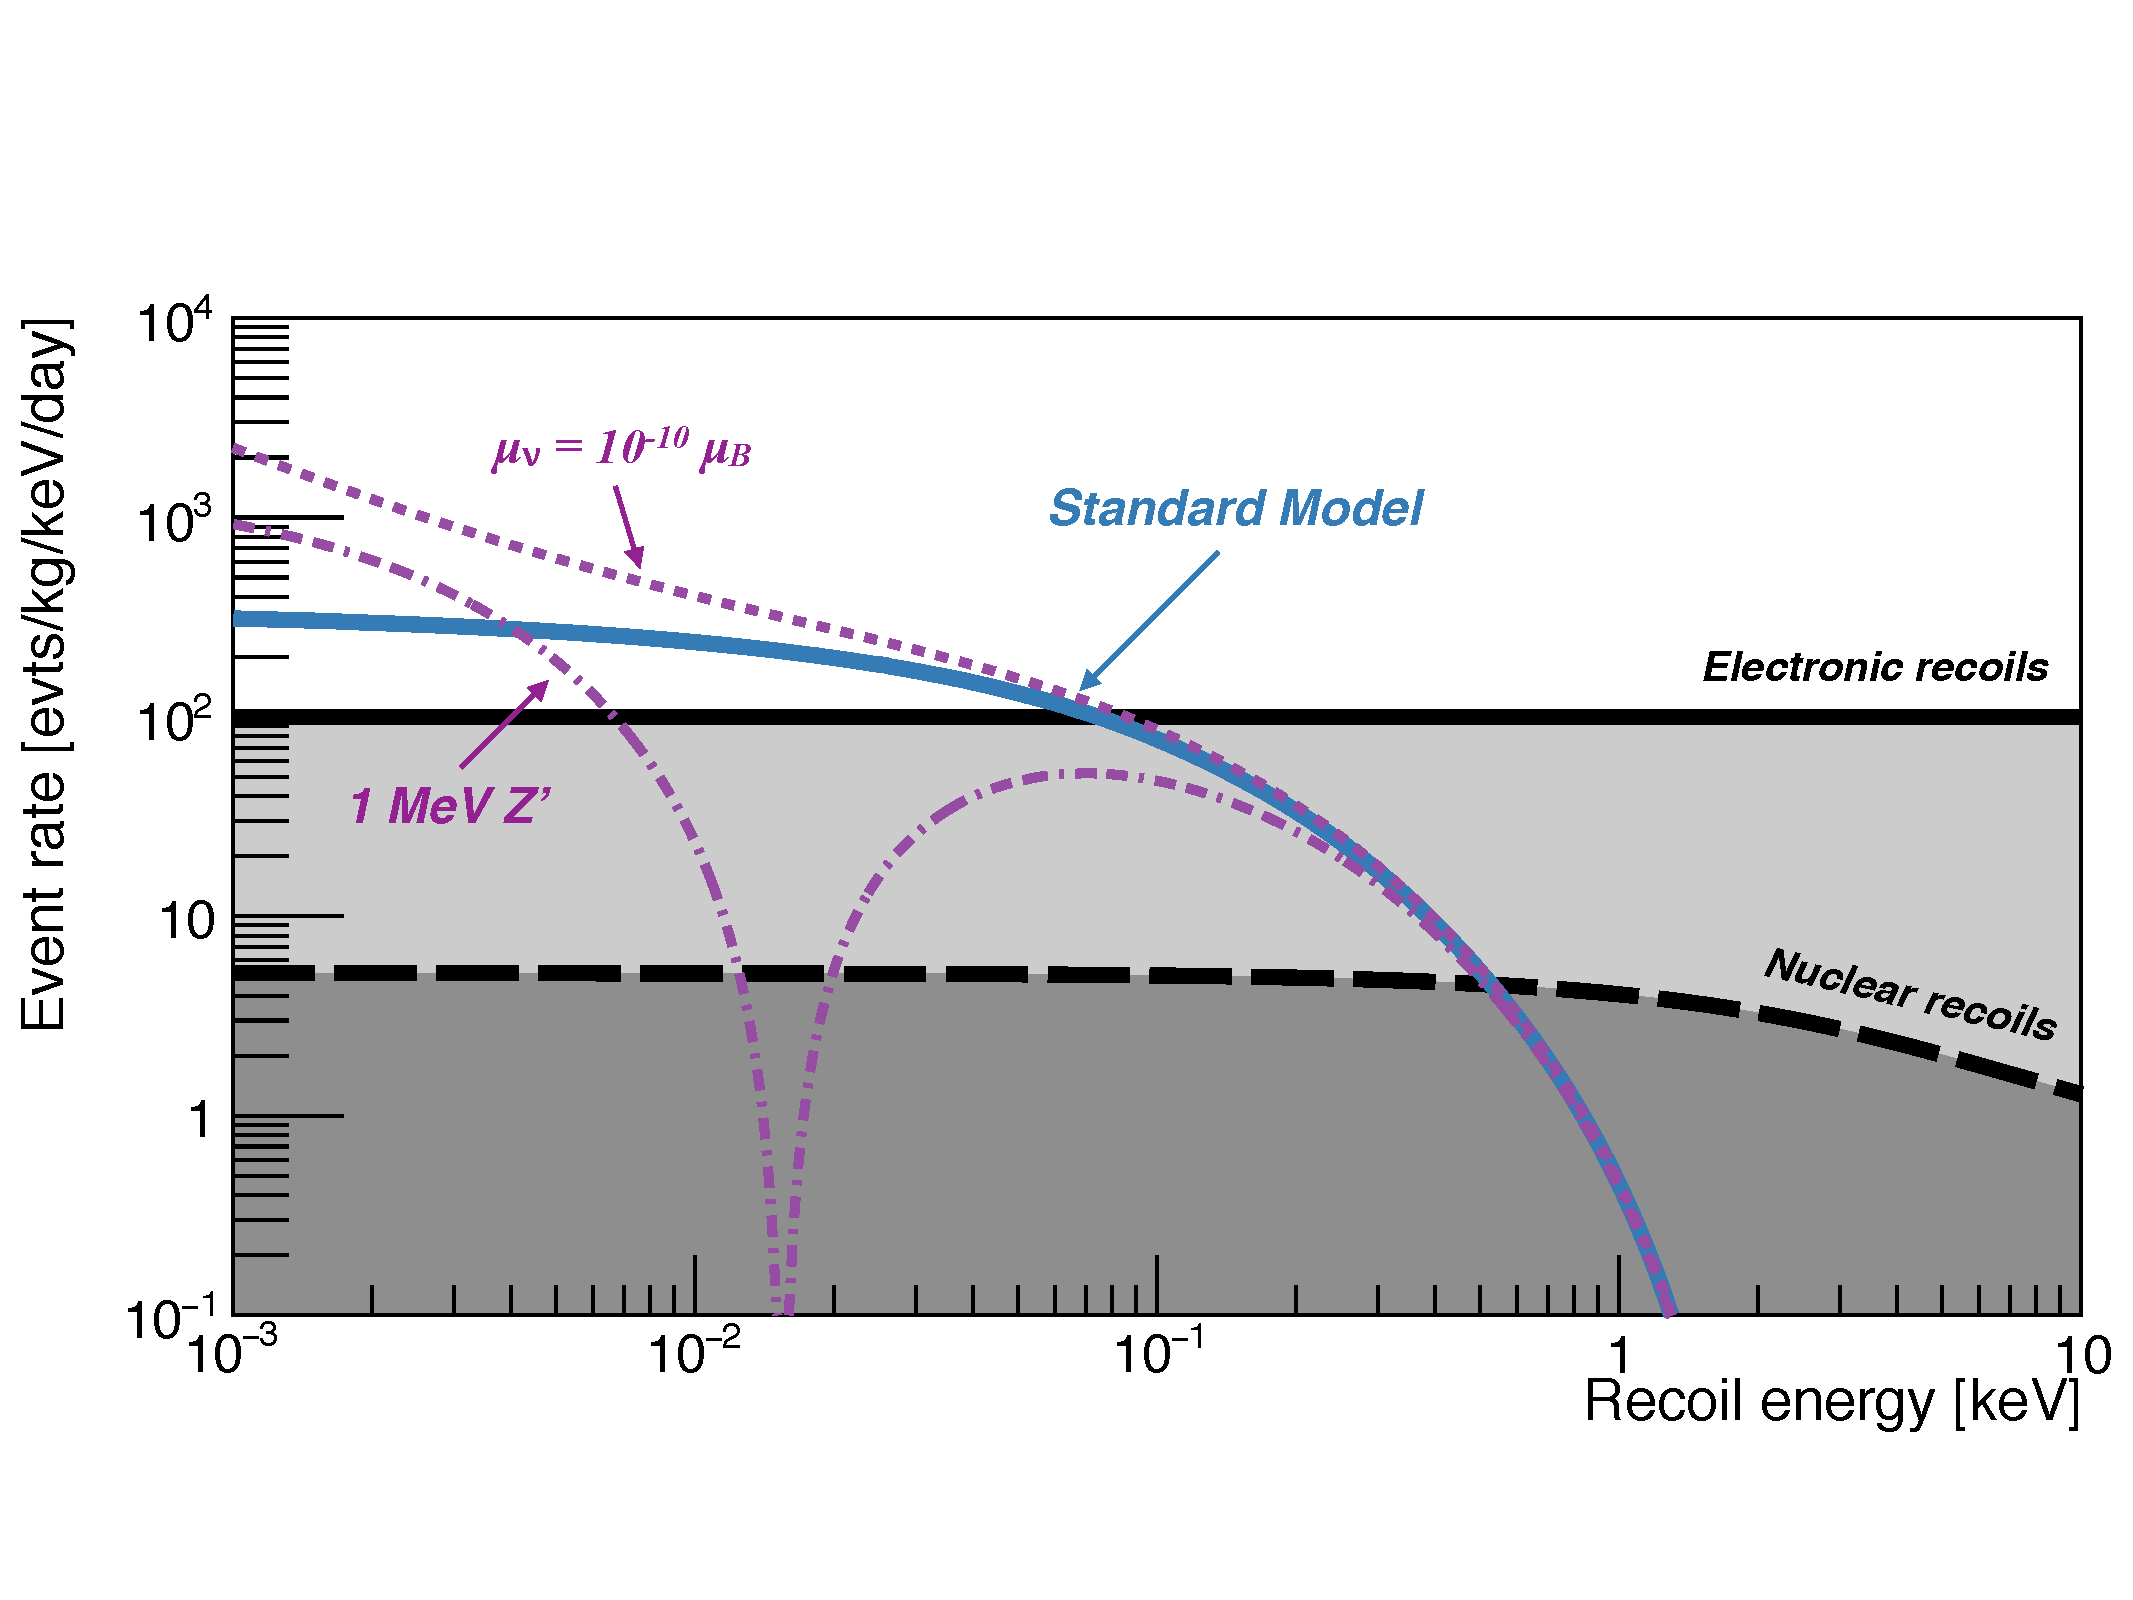
\includegraphics[width=0.7\textwidth]{Figures/Introduction/cenns_spectrum_ill.pdf}
\caption{Simulation of the background noise on the CENNS spectrum for \Ricochet{} at the ILL. The radioactive background noise is represented as its two components inducing electronic recoils in light grey and inducing nuclear recoils in dark gray. Figure taken from \cite{Billard:2018jnl}.}
\label{fig:cenns-new-physics}
\end{figure}

We can notice that the spectrum is given in \si{events \per \kilo\eV \per \kg \per \day} and therefore to have a sufficient statistic it is necessary to find an interesting ratio of detector mass over data acquisition time.

% One can quote for example the dark matter research experiment XENON1T which uses a detector whose total mass is greater than one ton and its version in development XENONnT which aims to go even further in terms of mass. This detector technology, based on a liquefied noble gas, is not the most efficient for the CENNS but above all requires a large experimental volume that is difficult to obtain near a nuclear reactor.
%Other technologies such as SuperKAMIOKANDE or Borexino neutrino experiments would be theoretically possible but the experimental volume would remain an impossible constraint to reconcile with the proximity to the nuclear reactor.
%The opposite approach consists in taking a low detector mass, which is easier to install, operate, analyze and protect from external background noise, and collecting experimental data for a long time. In theory there would be no problem to this, but in practice the non-stationarity of the noise, the volume of the data, the time to analyze this data and the time of experiment (mobilization of human resources, technical, infrastructure, ...) make the task very difficult. There is therefore a compromise to be made between the mass of the detector and the desired duration of data acquisition for a given number of CENNS events.

Having an ultra massive detector near the nuclear core represents a real technical challenge, and it is hardly possible to achieve significantly lower energy thresholds.
The exposure of the detector, which is its mass multiplied by the experiment time in \si{\kg \day}, is not the only parameter to be considered, it is necessary to have sufficient sensitivity to measure the minute energy deposition generated by the interaction of a neutrino with matter. This is the reason why the \Ricochet{} collaboration chose to use low-threshold cryogenic bolometers.
% able to differentiate between nuclear and electronic recoils in order to increase the signal-to-noise ratio (as suggested by numerical simulations).
To carry out the identification of neutrino recoils, the material of the target for coherent neutrino scattering is semiconductor germanium which features an intrinsic discrimination ability thanks to a recoil heating and ionizing this material. The double energy measurement, described later in the section \ref{sec:detector-principle}, leads to difference in signal signature between nuclear recoils, produced by CENNS, and electronic recoils generated by the electronic component of the background.

% one way to do this is to measure the temperature increase induced by a deposit of energy while measuring the electron-hole pairs created in the semiconductor material that serves as a target for coherent elastic scattering. ]???

Specifically, a detector with the following characteristics would be required:
\begin{itemize}
	\item detection threshold / energy resolution: $E_R \sim \SI{50}{\eV}$ / $\sigma(E_R) \sim \SI{10}{\eV}$,
	\item ability to discriminate between electronic and nuclear recoils with thermometer + electrodes for electronic background rejection with semiconductor material ,
	\item mass of the detector: $m_d \sim \SI{1}{\kg}$ with a flux of \SI{e12}{\cm^{-2} \s^{-1}} to have about ten of CENNS events per day.
\end{itemize}

To meet these specifications, the members of the \Ricochet{} collaboration are developing an innovative detector called CryoCube which is presented in the figure \ref{fig:cryocube}. It will be composed of 27 germanium crystals of \SI{38}{\g} each equipped with a heat measurement channel and an ionization measurement channel for discrimination purpose. The goal of my thesis is the design of the elementary cryogenic detectors.

\begin{figure}
\centering
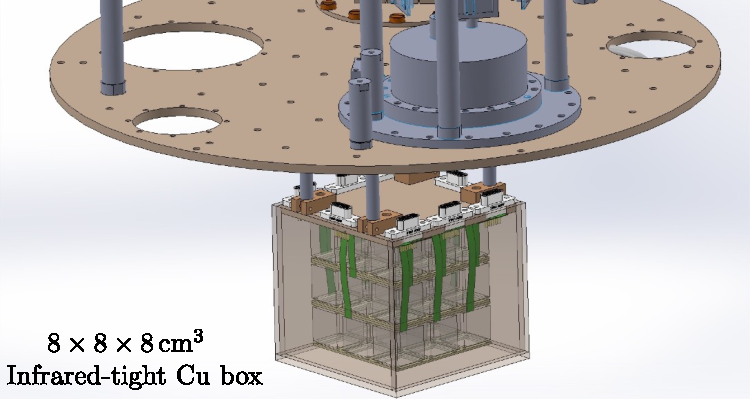
\includegraphics[scale=1]{Figures/Introduction/cryocube.pdf}
\caption{3D model of the CryoCube installed at the coldest stage of its cryostat. We can see by transparency the 27 germanium crystals of 38g electrically connected to the systems of acquisition by the green cables.}
\label{fig:cryocube}
\end{figure}


